\documentclass[a4paper, 12pt, fleqn]{article}
\usepackage{libertine}
% \usepackage{setspace}%\setstretch{1.24} %Zeilenabstand �ndern
\usepackage[utf8]{inputenc} %Umlaute&Sonderzeichen einlesbar
\usepackage[normalem]{ulem}
\usepackage{amsmath,amssymb,amsthm}
\theoremstyle{definition}
\newtheorem{hyp}{H} 
\usepackage{natbib}
\setcitestyle{notesep={; }}

\usepackage[pdfborder={0 0 0}, breaklinks=true]{hyperref}
\usepackage{microtype}
\usepackage{booktabs}
\usepackage{graphicx}
\usepackage{pdflscape}
\usepackage{float}
\usepackage{pdfpages}
\usepackage{floatflt}
\long\def\symbolfootnote[#1]#2{\begingroup%
\def\thefootnote{\fnsymbol{footnote}}\footnote[#1]{#2}\endgroup}
\usepackage{array}
\newcommand{\inew}[1]{{\color{blue} #1\color{black}}}
\usepackage{comment}
\specialcomment{icomm}{\color{red}\footnotesize [\textsc{iren}: }{] \normalsize\color{black}}
\newcommand{\iout}[1]{{\color{red}\sout{#1}}}
%}
\newcommand{\old}[1]{{\color{lightgray} #1\color{black}}}

\newcommand{\mytitle}{{\Large \textsc{When personalization deters delegation to algorithms: Evidence from a preregistered experiment}}}

%opening
\title{\mytitle}
%\author{Wania Lefuloff}
\date{}

%Fuer Zeilenabstand
\usepackage{setspace}
%\doublespacing

%Fuer 1.5 inch margins
%\usepackage[a4paper]{geometry}
%\geometry{top=1.5in, bottom=1.5in, left=1.2in, right=1.2in}

\begin{document}
 
%  \maketitle
\thispagestyle{empty}
\begin{center}
  \mytitle\symbolfootnote[4]{We are grateful to all the many people who helped us write this paper, first and foremost Chris Starmer and Robin Cubitt, to whom we owe several aspects of the design, as well as the lively research group at the TWI and participants of numerous workshops and conferences.}
  \vspace{.55cm}\\
 Lara Suraci \qquad\qquad\qquad Irenaeus Wolff\symbolfootnote[3]{Corresponding author. Thurgau Institute of Economics, Hafenstrasse 6, 8280 Kreuzlingen, Switzerland, \textit{wolff@twi-kreuzlingen.ch}.}
\\\vspace{.25cm}
 \begin{small}
  \phantom{mortext}\textit{DG Cities \qquad\qquad Thurgau Institute of Economics \\ \phantom{moretext}\phantom{University} \qquad\qquad (TWI) / University of Konstanz} %University of Konstanz\\ Hafenstrasse 6, 8280 Kreuzlingen, Switzerland\\ wolff@twi-kreuzlingen.ch}
  \vspace{.03cm}\\
\vspace{.6cm}
 {This version: 30$^{\text{th}}$ March, 2026}
\vspace{.6cm}
\end{small}
\end{center}

\begin{abstract}
  Algorithmic decision aids increasingly act on users’ behalf, and in many instances users can either retain control or delegate decisions to an algorithm. We test whether preference-based personalization increases or decreases willingness to delegate compared with an objective optimization criterion. In a preregistered between-subjects experiment (N = 233), participants repeatedly chose whether to decide themselves or to delegate to an algorithm. In one treatment, the delegation option is an optimization-based algorithm selecting the option with the highest expected value. In the other treatment, it is a preference-based (personalized) algorithm selecting according to participants’ previously elicited preferences. We find no evidence that preference-based personalization increases delegation relative to expected-value optimization throughout the task. Instead, personalization deters delegation in two ways. First, at first contact participants are significantly less likely to delegate to the preference-based algorithm than to the optimization-based algorithm; this difference is confined to the very first decision and disappears immediately thereafter, with delegation rates statistically indistinguishable across algorithm types in subsequent decisions. Second, categorical non-delegation (never delegating) is substantially more prevalent under preference-based personalization (15.7\%) than under objective optimization (3.4\%). 
  Taken together, the results are consistent with the idea that preference-matching can raise initial hesitation and heighten agency- and responsibility-related concerns for a subset of users, functioning as an acceptance barrier even when personalization is normatively appealing.
  
     \vspace{.25cm}
  \textit{Keywords:} {AI delegation, human-AI delegation, personalization, algorithm appreciation, algorithm aversion, trust in AI, financial decision-making, preregistered experiment.}\vspace{.15cm}
  \\\textit{JEL:} {D81, C91, D83}
\end{abstract}
\vspace{-.5cm}

\section{Introduction}\label{sec:intro}
Algorithmic systems increasingly make and implement decisions on users’ behalf in both everyday and high-stakes contexts, from automated driving and financial robo-advising to autonomous trading and smart-home control. Public perceptions of algorithmic decision-making vary substantially across domains and are shaped by perceived legitimacy and accountability \citep{Aysolmaz2023}. In many such settings, users face a concrete choice: they can retain control and decide themselves, or delegate the decision to an algorithm. Delegation can reduce cognitive effort and simplify complex choice tasks, but it can also reshape perceived agency and responsibility for outcomes. Recent literature shows that people do delegate consequential choices to AI systems, yet such delegation is psychologically nuanced and sensitive to characteristics of the decision maker \citep{Candrian2022}. Note that throughout the paper, we use the term ``algorithmic decision aid'' broadly to include both rule-based algorithms and AI-based systems. This reflects the practical reality that, from a user's perspective, the boundary between ``AI'' and other algorithmic decision rules is often opaque.

A common assumption is that \emph{personalization} should increase acceptance. If individuals differ in preferences, then a decision aid that incorporates those preferences should, in principle, deliver higher subjective utility than a one-size-fits-all rule. In financial decision support, for example, systems often elicit risk preferences and translate them into portfolio recommendations. Yet acceptance of robo-advisory tools has often been examined in terms of perceived usefulness, ease of use, trust, and adoption intention, rather than in terms of how personalization itself shapes willingness to delegate \citep{Figa-Talamanca2022,Mahmud2025}.

However, behavioral evidence suggests that willingness to use algorithmic advice is not determined by instrumental considerations alone. People sometimes avoid algorithms and sometimes prefer them, depending on context and perceived role \citep{Dietvorst2018,Logg2019}. They also interpret and rationalize recommendations rather than mechanically follow them \citep{Yeomans2019}, and interdisciplinary syntheses emphasize that acceptance depends on multiple moderators \citep[including perceived control;][]{Mahmud2022,Chugunova2022}. 

Preference-based personalization can therefore be double-edged: while it promises better fit, it can also make decisions traceable to a user profile, potentially heightening discomfort with being categorized or increasing perceived responsibility for outcomes (``it chose based on me'').
In our data, however, post-task responses indicate that many non-delegators explicitly report wanting to keep responsibility and control, suggesting that resistance is not simply a preference for offloading accountability. Consistent with this broader perspective, recent evidence shows that increased transparency can backfire by triggering negative social interpretations and reducing acceptance \citep{Chen2024}, and that transparency can produce resistance rather than compliance in algorithmic management contexts \citep{Hu2024}. Related work further argues that acceptance of automated decision-making depends less on whether a system is treated as an ``agent'' and more on perceived benefits and perceived control \citep{Schaap2024}.

These issues are especially salient at first contact, when users have no experiential basis for evaluating an algorithm. In repeated interaction settings, people can quickly settle into stable interaction strategies, and overreliance (and its costs) can emerge even when performance information is available \citep{Klingbeil2024}. Moreover, reactions to algorithmic errors can be persistent \citep{Renier2021}, suggesting that expectations about how an algorithm will behave may matter disproportionately early on. Importantly, behavioral reliance and self-reported trust need not coincide: evidence from AI-advisor interactions shows that determinants of behavioral trust can diverge from self-reported trust \citep{Schreibelmayr2025}. This motivates our focus on observable delegation behavior rather than attitudes alone.

Finally, autonomy considerations are themselves a driver of acceptance: increasing user autonomy can increase recommendation acceptance \citep{Fink2024}, and preferences for decision autonomy can constrain delegation even when delegation is instrumentally attractive \citep{Ivanova-Stenzel2025}. Together, this motivates studying delegation as an observable behavior and treating first contact as a critical moment when abstract cues about an algorithm's decision logic may dominate.

In this study, we contrast two decision rules that are both plausible in financial choice settings but may elicit different reactions. One algorithm follows an \emph{objective optimization rule} and selects the option with the highest expected value (EV), which may appear impersonal and easier to justify as a rule-based benchmark. The other is \emph{preference-based personalization} in a narrow sense: it predicts choices from each participant's previously elicited preferences rather than maximizing EV. In implementation terms, the personalized algorithm maps each participant's earlier choices in a simpler elicitation environment to corresponding choices in a more complex environment later in the experiment; it does not involve adaptive updating or learning during the delegation task.
The central question is whether people are more willing to delegate to EV maximization than to preference-based personalization. This comparison connects to work showing that delegation can serve responsibility-sharing motives \citep{Kirchkamp2019} and to recent studies on financial advisor choice and responsibility attribution in delegation settings \citep{Ismagilova2025,Werner2026}.

\subsection*{Preregistered hypothesis and analysis plan}
Consistent with our preregistration ({\scriptsize\url{https://aspredicted.org/7un5qf.pdf}}), the main hypothesis is: 
\begin{hyp}
	People are more likely to delegate financial decisions to an EV-maximizing algorithm than to a personalized algorithm that incorporates their (revealed) preferences.
\end{hyp}

Our preregistered primary analyses test this hypothesis in two complementary ways. First, we test the treatment difference in delegation in the first decision (round 1) using a one-sided Boschloo exact test. This isolates first contact, when participants have no outcome feedback and must decide whether to delegate based on their interpretation of the algorithm. Second, we test whether EV maximization leads to higher delegation overall by comparing participants' average delegation frequencies across rounds using a one-sided Wilcoxon--Mann--Whitney test.

To account for the repeated-decision structure and additional determinants of delegation, our preregistration also specifies a multivariate regression analysis. We estimate a model with treatment indicators interacted with the decision period, decision-ID fixed effects, and participant-clustered standard errors. We further include the feedback history in the form of including the share of zero outcomes among prior delegated choices, to control for how experienced payoffs may influence subsequent delegation decisions. This preregistered specification tests whether any treatment difference varies systematically over decisions while controlling for option-set heterogeneity and participants' feedback histories.

\subsection*{Study overview and supplementary analyses}
We implement this design in a between-subjects experiment in which participants repeatedly choose whether to decide themselves or delegate to the assigned algorithm. The repeated-decision setting provides a direct behavioral measure of delegation and allows us to distinguish first-contact delegation from later decisions made after minimal experience.

In addition to the preregistered tests, we report a small set of analyses to characterize heterogeneity in delegation propensity. In particular, we examine categorical non-delegation (never delegating across rounds). This outcome captures a distinct form of resistance to algorithmic control transfer and is relevant for understanding which users may opt out of decision aids altogether.

In sum, this paper provides a preregistered test of a simple but consequential claim: even in a setting where preference-based personalization may appear normatively attractive, people may nonetheless be more willing to delegate to a `more objective' algorithm. Our design and preregistered analyses allow us to assess this claim both at first contact and on average across repeated decisions, and show that resistance to personalization can take the form of both first-contact hesitation and categorical non-delegation.




%A common assumption is that personalization should increase acceptance. If individuals differ in preferences, then a decision aid that incorporates those preferences should, in principle, deliver higher subjective utility than a one-size-fits-all rule. In financial decision support, for example, systems often elicit risk preferences and map them to recommended portfolios. However, behavioral evidence suggests that willingness to use algorithmic advice is not determined by instrumental considerations alone. People sometimes avoid algorithms, sometimes prefer them, and often react to how they interpret a system’s role and legitimacy (e.g., Dietvorst et al., 2015; Logg et al., 2019; Castelo et al., 2019). Preference-based personalization can therefore be double-edged: while it promises better fit, it can also make the system’s decisions traceable to a user profile, potentially heightening discomfort with being categorized or increasing perceived responsibility for outcomes (“it chose based on me”).
%
%These issues are especially salient at first contact, when users have no experiential basis for evaluating an algorithm. At first contact, delegation is likely to depend on abstract cues about what an algorithm optimizes and what that implies about the user, rather than on experienced accuracy. Therefore, early impressions and system descriptions can shape adoption and reliance even when objective performance is held constant (e.g., Kosch et al., 2022). Moreover, self-reported trust and behavioral reliance often diverge (Papenmeier et al., 2022), which motivates studying delegation as an observable behavior rather than equating it with stable trust. 
%
%In this study, we contrast two decision rules that are both plausible in financial choice settings but may elicit different reactions. One algorithm selects the option with the highest expected value (EV), a rule that may appear impersonal and objectively justified. The other is preference-based (“personalized”) in a narrow sense: it selects options according to participants’ previously elicited (revealed) preferences rather than by optimizing EV. Here, “personalized” refers to profile-based selection from elicited preferences, not to online learning or continuous adaptation. The central question is whether people are more willing to delegate to EV maximization than to preference-based personalization.
%
%Preregistered hypothesis and analysis plan
%
%Consistent with our preregistration, the main hypothesis is:
%
%H1 (Preregistered). People are more likely to delegate financial decisions to an EV-maximizing algorithm than to a personalized algorithm that incorporates their (revealed) preferences.
%
%Our preregistered primary analyses test this hypothesis in two complementary ways. First, we test the treatment difference in delegation in the first decision (round 1) using a one-sided Boschloo exact test. This isolates first contact, when participants have no outcome feedback and must decide whether to delegate based on their interpretation of the algorithm. Second, we test whether EV maximization leads to higher delegation overall by comparing participants’ average delegation frequencies across rounds using a one-sided Wilcoxon–Mann–Whitney test.
%
%To account for the repeated-decision structure and additional determinants of delegation, our preregistration also specifies multivariate regression analyses. We estimate models with treatment indicators interacted with the decision period, decision-ID fixed effects, and participant-clustered standard errors. We further include measures capturing feedback history, including the share of zero outcomes among prior delegated choices, to control for how experienced payoffs may influence subsequent delegation decisions. This preregistered specification tests whether any treatment difference varies systematically over decisions while controlling for option-set heterogeneity and participants’ feedback histories.
%
%Study overview and supplementary analyses
%
%We implement this design in a preregistered between-subjects experiment in which participants repeatedly choose whether to decide themselves or delegate to the assigned algorithm. The repeated-decision setting provides a direct behavioral measure of delegation and allows us to distinguish first-contact delegation from later decisions made after minimal experience.
%
%In addition to the preregistered tests, we report a small set of analyses to characterize heterogeneity in delegation propensity. In particular, we examine categorical non-delegation (never delegating across rounds). This outcome captures a distinct form of resistance to algorithmic control transfer and is relevant for understanding which users may opt out of decision aids altogether. 
%
%In sum, this paper provides a preregistered test of a simple but consequential claim: even in a setting where preference-based personalization may appear normatively attractive, people may nonetheless be more willing to delegate to an EV-maximizing algorithm. Our design and preregistered analyses allow us to assess this claim both at first contact and on average across repeated decisions, and show that resistance to personalization can take the form of both first-contact hesitation and categorical non-delegation.


\section{Related Work}
\label{sec:related}

Our work sits at the intersection of literatures on (i) behavioral uptake of algorithmic decision aids, (ii) delegation and responsibility in human--algorithm interaction, and (iii) personalization and transparency as acceptance levers that may also create resistance. Below, we situate our preregistered comparison of an EV-maximizing algorithm versus a preference-based (personalized) algorithm within these streams.

\subsection{Algorithm aversion, appreciation, and conditions for uptake}
A central starting point is the mixed evidence on whether people follow algorithmic advice. Seminal work on \emph{algorithm aversion} shows that people may avoid algorithms after observing them err, even when the algorithm performs well in expectation \citep{Dietvorst2018}. Subsequent research documents also cases of \emph{algorithm appreciation} (in which people prefer algorithmic to human judgment) and highlights that adoption depends on context and comparison standards \citep{Logg2019}. In addition, people actively interpret and rationalize recommendations, which can affect whether they use them and how they integrate them with their own judgment \citep{Yeomans2019}. A recent systematic review synthesizes this body of work and emphasizes moderators that shape the direction and magnitude of aversion/appreciation effects \citep{Mahmud2022}. More broadly, an interdisciplinary review of experiments on human--machine interaction provides additional integration across disciplinary boundaries and underscores how acceptance depends on what the machine is perceived to be doing and for whom \citep{Chugunova2022}. 
Together, this literature motivates our focus on a concrete behavioral outcome---delegation---and on how the \emph{decision rule} (objective EV maximization vs preference-based personalization) shapes willingness to hand over control to an algorithm.

\subsection{Delegation, agency, and responsibility sharing}
Delegation differs from merely receiving advice: it is a choice to transfer control to another actor (here, an algorithm) and is therefore closely tied to perceived agency and responsibility. Empirical work on delegation to autonomous AI demonstrates that people do not evaluate expected payoffs alone; they also consider what handing over a decision means for ownership of the choice and its consequences \citep{Candrian2022}. Complementing this, work on responsibility sharing suggests that decision-makers may strategically value distributing or externalizing accountability to a machine \citep{Kirchkamp2019}. Related studies in organizational and leadership contexts similarly show that perceptions of legitimacy, competence, and responsibility affect acceptance of algorithmic decision-makers \citep{Hoeddinghaus2021}. Recent work on choosing between human and algorithmic advisors further points to responsibility sharing as a key determinant of advisor choice \citep{Gazit2023}. A complementary perspective comes from work on \emph{human-in-the-loop} designs: allowing human involvement can increase uptake but may reduce decision accuracy, underlining that control allocation shapes behavior and outcomes \citep{Sele2024}. Finally, preference for decision autonomy has been theorized and empirically examined as a stable individual tendency that can constrain algorithm adoption, even when delegation would increase expected payoff \citep{Ivanova-Stenzel2025}. These strands provide a natural backdrop for our preregistered hypothesis that delegation may be higher for an impersonal, EV-maximizing rule than for a preference-based rule that is explicitly tied to the participant's own profile.

\subsection{Personalization as an acceptance lever---and as a potential barrier}
Personalization is often assumed to increase acceptance by aligning system behavior with users' preferences. However, several streams suggest that personalization can also create resistance by increasing perceived self-relevance, profiling concerns, or accountability. In algorithmic recommendation settings, opening the ``black box'' can backfire when it induces meta-level social interpretations (e.g., feelings of being judged or dehumanized), which in turn reduce acceptance \citep{Chen2024}. Work on algorithmic management similarly points to a transparency--resistance paradox, showing that providing more explicit information about how recommendations are generated can sometimes increase pushback rather than compliance \citep{Hu2024}. In addition, recent work emphasizes that acceptance is shaped less by whether a system is an ``agent'' per se and more by perceived benefits and control \citep{Schaap2024}. For our setting, this is directly relevant because preference-based personalization can be interpreted as threatening autonomy or reducing subjective control over the decision process, even when it is normatively well-matched to individual preferences.

\subsection{Transparency, explainability, and reliance behavior}
A large literature studies whether transparency and explainability increase trust, reliance, and compliance with AI outputs. The ``algorithmic affordance'' perspective emphasizes fairness, accountability, and transparency as drivers of how users interpret and engage with algorithmic systems \citep{Shin2019}. Experimental work shows that explainable AI can shift both trust and behavior, especially in higher-stakes decision tasks \citep{Leichtmann2023}. Work on decision control and explanations in human--AI collaboration finds that giving users more control (and appropriately designed explanations) can improve perceptions and compliance \citep{Westphal2023}. In applied decision-support contexts, transparency affects advice utilization through psychological mediators such as trusting beliefs and perceived understanding \citep{Ning2024}. Importantly, transparency effects may depend on whether system performance meets expectations: when outcomes confirm expectations, transparency can play a different role than when they do not \citep{Sun2026}. These findings motivate our preregistered analysis that accounts for feedback histories (e.g., the share of zero outcomes among prior delegated choices) and decision periods, because experienced outcomes are a central driver of subsequent reliance.

\subsection{Contextual and individual-difference moderators of trust and delegation}
Recent work increasingly emphasizes heterogeneity: algorithm uptake varies across people, tasks, and situational constraints. An experimental study of overreliance documents both the extent and the potential costs of relying too heavily on AI \citep{Klingbeil2024}. Complementing this, research on user autonomy shows that allowing users to decide can increase acceptance of recommendations, suggesting that autonomy concerns can be a primary driver of behavior \citep{Fink2024}. Personality and context also shape delegation and collaboration with algorithms \citep{Ferraz2025}. Task properties matter as well: trust and reliance vary with task objectivity, time pressure, and cognitive load \citep{Yang2025}. More generally, psychological readiness has been proposed as a determinant of whether people are willing to accept algorithmic advice at all \citep{Kim2026}. Additional evidence on trust formation in AI-advisor interactions, including in cooperative problem-solving contexts, highlights that self-reported and behavioral indicators need not coincide \citep{Schreibelmayr2025}. Recent evidence comparing loss and gain contexts suggests that individual loss aversion can moderate willingness to delegate to AI, further underscoring the importance of participant-level heterogeneity \citep{Werner2026}. These insights align with our decision to report not only average delegation but also categorical non-delegation as a practically important form of heterogeneity.

\subsection{Financial advice and robo-advisors as an application domain}
Although our task is experimentally stylized, it is close to a robo-advisor setting in which users choose whether to make portfolio-like decisions themselves or delegate to an algorithmic rule. Financial decision-making therefore provides a natural application context in which objective optimization and preference-based personalization are both prominent. Survey evidence shows that public perceptions of algorithmic decision-making vary systematically with domain and perceived legitimacy \citep{Aysolmaz2023}. In the robo-advisor literature, adoption has been studied across demographic segments \citep{Figa-Talamanca2022}, and newer work examines how users interpret and combine human and robo-advisor inputs in sequential decision settings \citep{Mahmud2025}. Additional studies compare delegation to human versus algorithmic financial advisors and emphasize responsibility and attribution concerns \citep{Ismagilova2025}. Related evidence examines when robo-advice improves financial decisions relative to self-directed choices \citep{Lambrecht2023}. Taken together, this literature motivates our application domain and suggests that differences in decision rules are likely to matter behaviorally, even when objective performance incentives are present.

\subsection{Synthesis and contribution}
Across these literatures, a recurring theme is that algorithm uptake is shaped by more than expected performance: it depends on perceived control, legitimacy, and how system behavior relates to the self \citep{Dietvorst2018,Logg2019,Chugunova2022}. Our study contributes a preregistered behavioral test of these ideas in a repeated-decision delegation paradigm, contrasting an EV-maximizing algorithm with a preference-based (personalized) algorithm. By jointly examining first-contact delegation, average delegation across rounds, and categorical non-delegation, we connect classic findings on algorithm aversion/appreciation with newer work on autonomy, transparency, and responsibility sharing \citep{Candrian2022,Gazit2023,Hu2024,Fink2024}.

\section{Method}
\label{sec:method}

\subsection{Participants and preregistered exclusions}
Participants were recruited via Prolific from a UK-based participant pool and completed the study online. The preregistered target was 120 participants per treatment condition before exclusions. We recruited N = 240 participants and then applied preregistered exclusion rules for data quality and protocol compliance. Exclusions covered failed bot/slider checks at first attempt, failed comprehension checks after the second attempt, failure to confirm careful participation, disclosed AI usage during the study, implausibly short completion times under the preregistered log-time rule, and incomplete data. The final analysis sample is N = 233 (EV condition: n = 118; preference-based condition: n = 115).

\subsection{Design and task}
The study used a between-subjects design with two algorithm conditions. In both conditions, participants completed a two-part experiment programmed in the online-ready version of z-Tree \citep{Fischbacher07}.

Part 1 consisted of 12 binary lottery choices used to elicit revealed risk preferences. Participants were truthfully told that "[t]he questions in this part are \textbf{hypothetical}, but the choices \textbf{may be meaningful for Part 2} (recall that your bonus payment from the experiment depends on what happens in Part 2)." The highlighted words were boldfaced in the original instructions. Options were ordered by payment amounts in Part 1 to ease comparison, as can be seen in the upper panel of Figure \ref{fig:example_screens}.

In Part 2, participants completed eight incentivized lottery decisions between eight lotteries each. The lottery decisions where connected to the first eight lottery decisions of Part 1 in the following way (the order of tasks was always fully randomized, except that the relevant decisions from Part 1 had to be the first eight decisions out of the 12 decisions in that Part). Figure \ref{fig:example_screens} showcases the relationship between the corresponding tasks. For the Part-2 task in the lower panel, we shuffled payments and states for each Option separately. Then, we
added three dominated Options for each of the initial Options, and finally changed the order in which the Options appeared on the screen. We chose not to randomize the orders to prevent tasks from becoming too easy, for example, due to all Options corresponding to one of the two dominating Options appearing without interruption. Even if such an ordering would have been unlikely ex ante, it could have made a participant aware of the construction principle of the Part-2 tasks, which is something that we strongly wanted to avoid.

\begin{figure}[htbp]
\centering
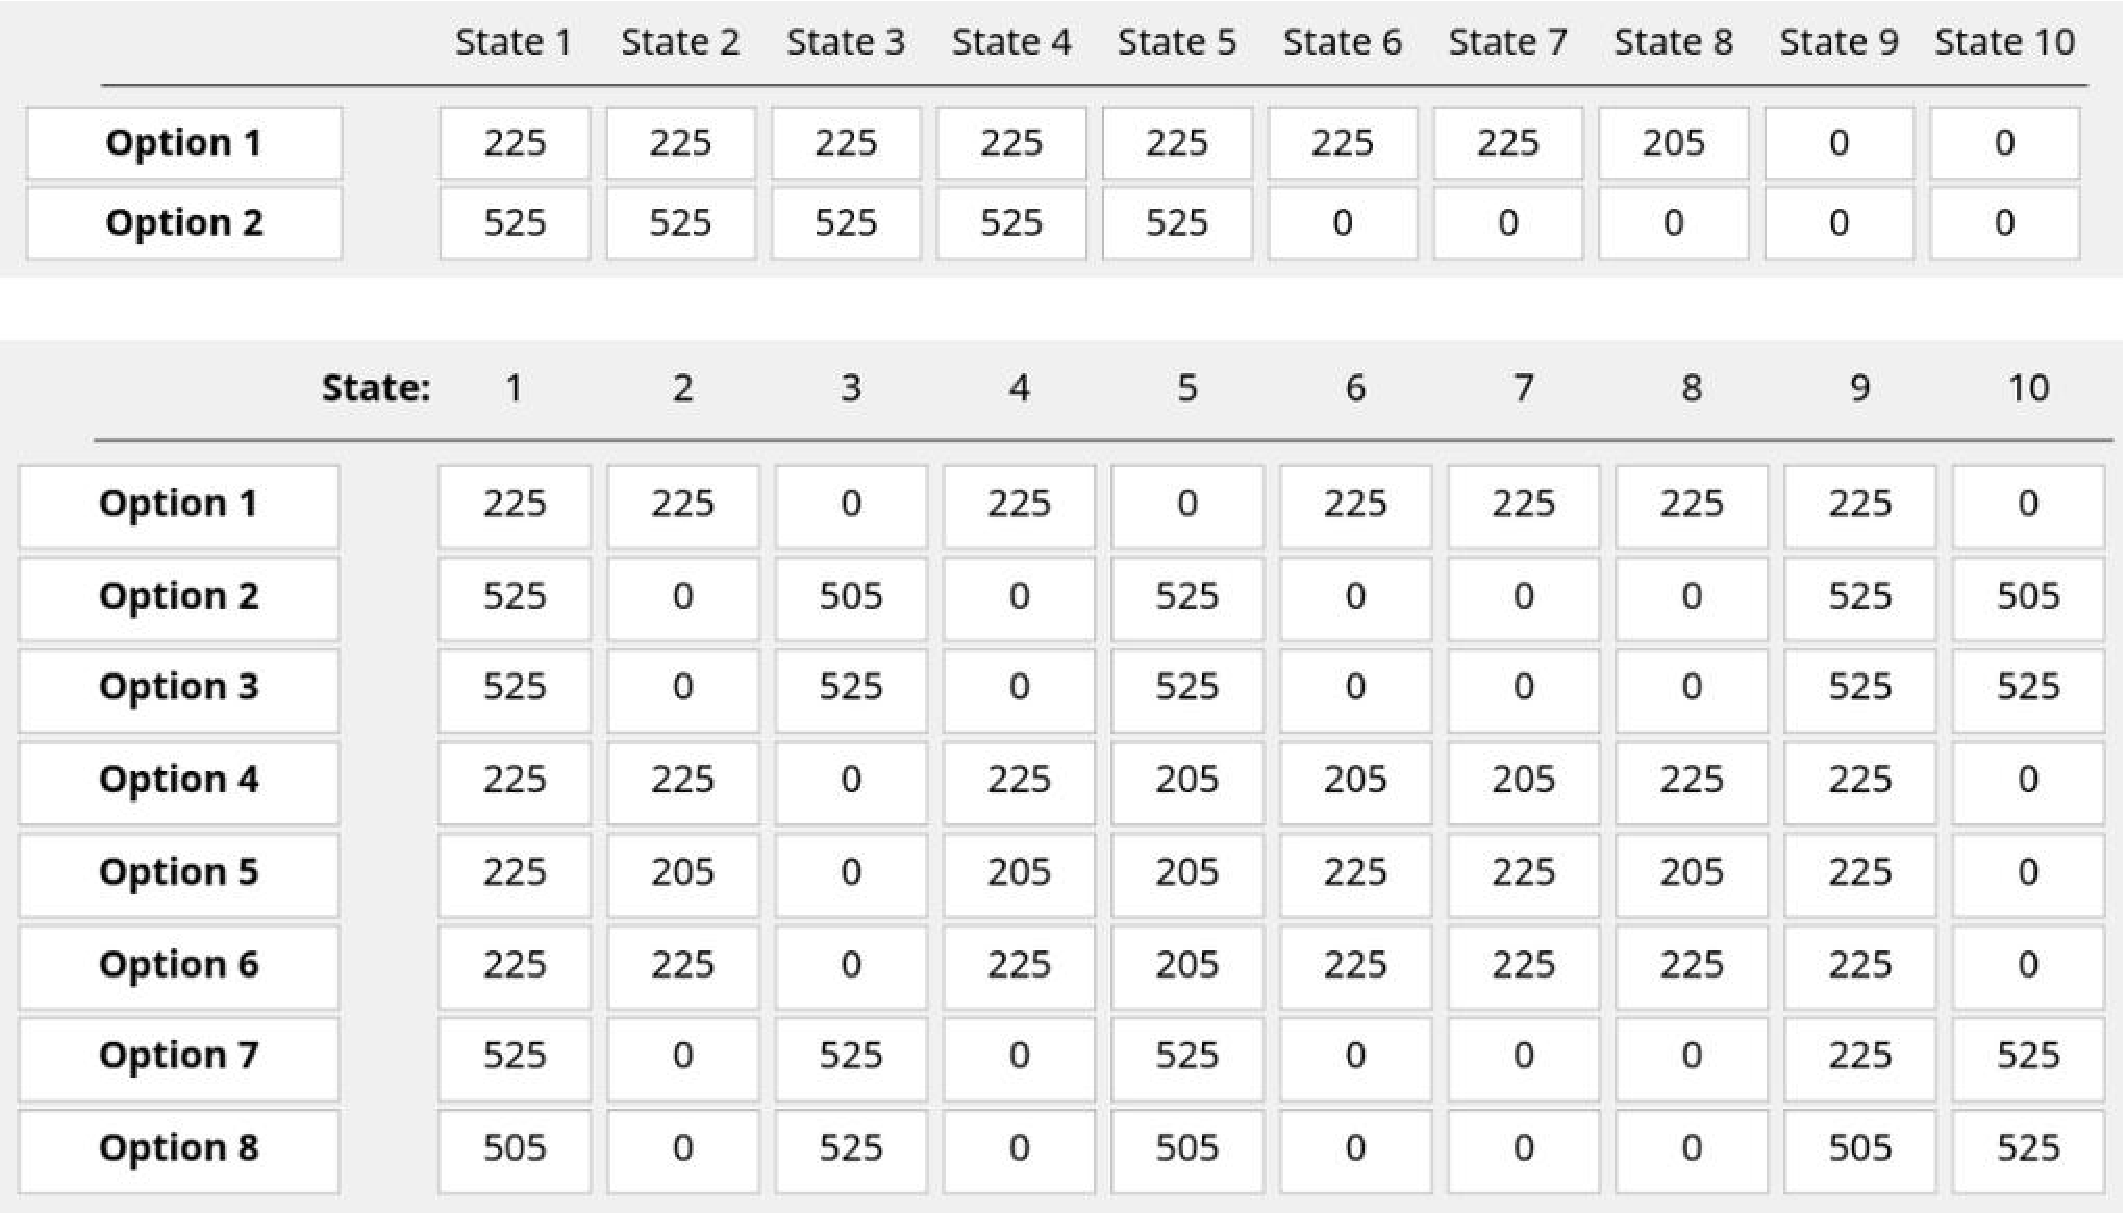
\includegraphics[width=0.85\textwidth]{Figure_ExampleScreens.pdf}
\caption{Example screens from Part 1 (preference elicitation, upper panel) and Part 2 (delegation decisions with lottery choices, lower panel).}
\label{fig:example_screens}
\end{figure}

The procedure for each round of Part-2 was as follows: Participants saw the full table for five seconds. Then, they saw a different screen on which they had five seconds to choose between delegating to the algorithm corresponding to their treatment condition and choosing an Option themselves.
In the EV condition, delegation selected the lottery with the highest expected value. In the preference-based condition, delegation followed each participant's elicited preference profile from Part 1 (i.e., profile-based personalization rather than online learning). Assignment to condition was randomized at the participant level.

If they did not delegate, they saw the table containing the eight Options for up to eight more seconds, during which they had to choose one of the Options. If they did not make a choice in the payoff-relevant choice, they did not earn a bonus payment from the experiment. The total payoff from the experiment was GBP 2.00 plus the points earned in one randomly selected round of Part 2, converted at a rate of 1 penny per point (participants could earn up to GBP 8.90 in addition to the base payoff). On average, participants earned GBP 4.14 including the base payoff for a median time of just under 16 minutes.

\subsection{Procedure}
After consent, participants completed attention and comprehension checks, then Part 1 (preference elicitation), followed by a question on how satisfied they were with their choices from Part 1. Then, participants completed Part 2 (delegation decisions with round-by-round outcome feedback), followed by a question of whether they would delegate to the algorithm in case they had to choose to delegate or not for 10 (hypothetical) additional tasks. Before the final post-task questionnaire containing demographics and attitudinal items, we asked them for self-reported reasons for their choice in the hypothetical choice at the end of Part 2. Because our theoretical focus is reliance behavior, primary outcomes are behavioral rather than attitudinal.

\subsection{Ethics approval}
The study received ethics approval from the Institutional Review Board of the Gesellschaft für experimentelle Wirtschaftsforschung e.V. (GfeW; German Association for Experimental Economic Research), certificate no. 19HBJNwQ (status: approved; expedited review; approval date: 11/13/2025; certificate validity through 11/13/2027; see {\footnotesize\url{https://gfew.de/ethik/19HBJNwQ}}). All participants provided informed consent before participation.

\subsection{Preregistered outcomes and analyses}
The preregistered hypothesis (H1) predicted higher delegation to the EV-maximizing algorithm than to the preference-based algorithm.
The preregistration document is available at {\footnotesize\url{https://aspredicted.org/7un5qf.pdf}}.

Primary preregistered analyses were:
\begin{enumerate}
  \item a one-sided Boschloo exact test for the treatment difference in delegation in round 1 (first contact), and
  \item a one-sided Wilcoxon--Mann--Whitney test comparing participant-level average delegation rates across Part 2.
\end{enumerate}

We additionally estimated preregistered linear probability models with decision-set fixed effects and participant-clustered standard errors, including treatment-by-period interactions and specifications excluding round 1.

\section{Results}
\label{sec:results}

\subsection{Overview}
Two empirical patterns organize the results. First, treatment differences are concentrated at first contact. Second, categorical non-delegation is substantially more common under preference-based personalization.

Choice quality among non-delegated decisions was low in both treatments. The share of non-dominated self-chosen options was 34.1\% in the EV condition and 35.1\% in the preference-based condition, implying that roughly two-thirds of self-made choices were dominated. Hence, participants had a clear instrumental reason to delegate.

\subsection{Primary test: first-contact delegation}
In round 1, delegation was higher in the EV condition than in the preference-based condition (66.9\% vs. 55.8\%). The preregistered one-sided Boschloo exact test yields p = 0.0413, supporting H1 for first-contact behavior.
Figure~\ref{fig:average_delegation_over_time} visualizes the round-level profile and shows that the treatment gap is concentrated in the first decision.

\begin{figure}[tb]
	\centering
	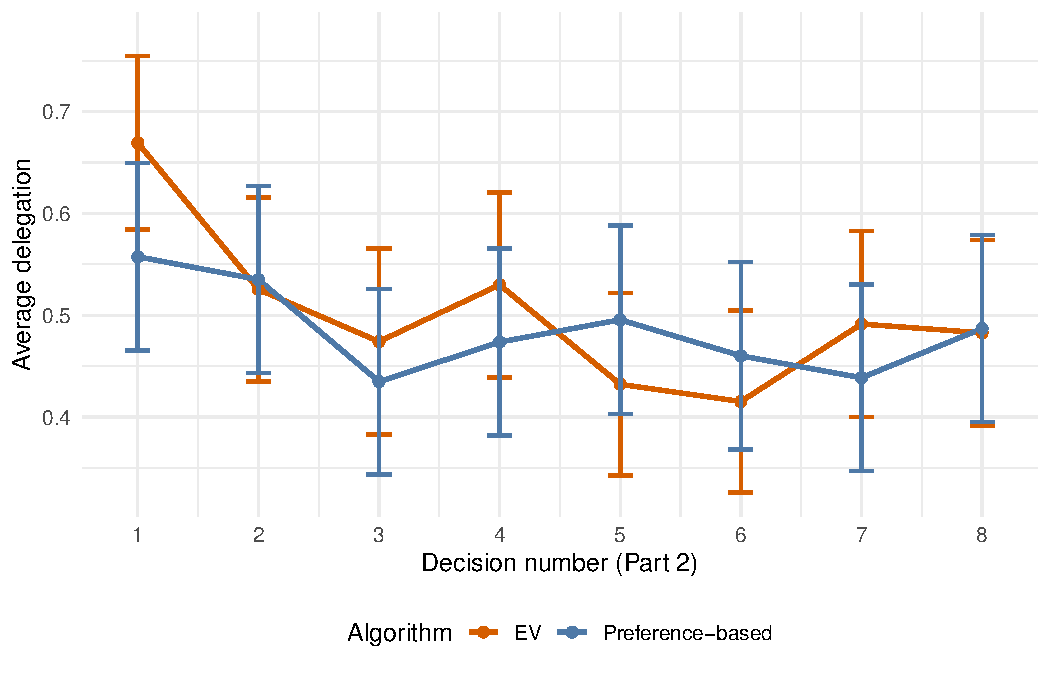
\includegraphics[width=0.8\textwidth]{Figure1_AverageDelegation.pdf}
	\caption{Average delegation over decisions in Part 2 by treatment condition.}
	\label{fig:average_delegation_over_time}
\end{figure}

\subsection{Primary test: delegation across repeated decisions}
At the participant level, the preregistered one-sided Wilcoxon--Mann--Whitney test on average delegation across Part 2 yields W = 6428 and p = 0.2425. We therefore do not find evidence of a treatment difference in average delegation across rounds.

The preregistered regression specifications points in the same direction. The EV coefficient equals 0.073 with SE = 0.053 and $p = 0.171$, and the interaction effect EV $\times$ period is negative (and imprecise, too: $\beta = -0.0123$, SE = 0.0083, $p = 0.138$), which suggests no difference across the whole of the experiment.\footnote{Running a regression with fixed effects for the task yields the same result as the Boschloo test, with $\beta = 0.113$, SE = 0.065, and $p = 0.041$ (one-sided).}

Taken together, the preregistered tests indicate that the treatment effect is concentrated at first contact and does not persist over repeated decisions. The convergence in delegation behavior over rounds is visible in Figure~\ref{fig:average_delegation_over_time}; the cross-participant distribution is shown in Figure~\ref{fig:delegation_ecdf}.

\begin{figure}[tb]
	\centering
	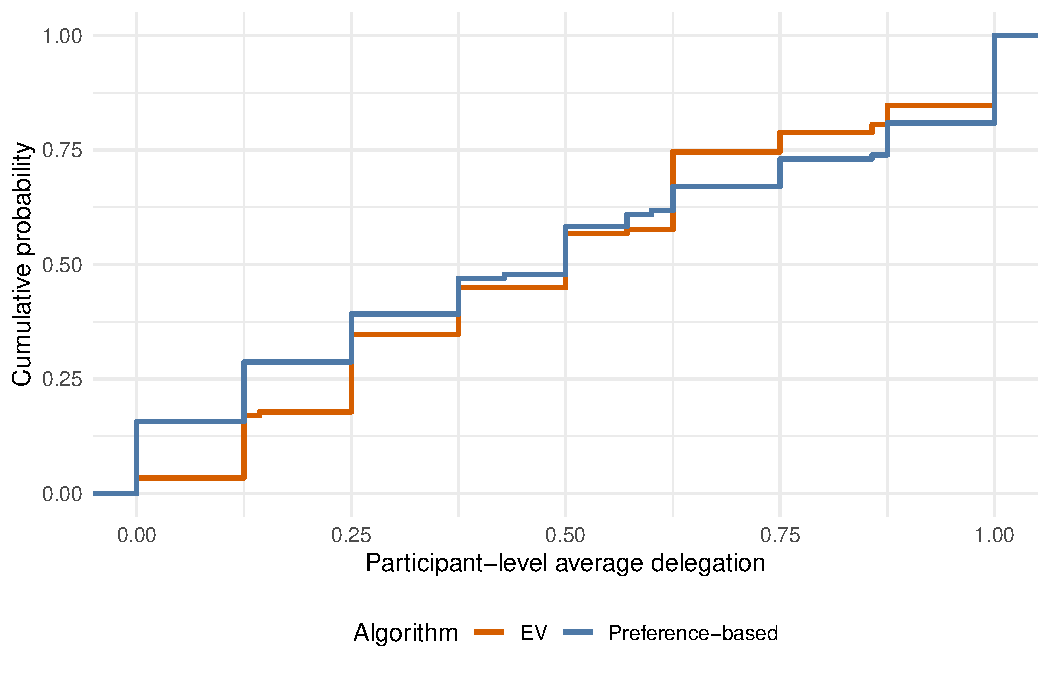
\includegraphics[width=0.78\textwidth]{Figure3_ECDF.pdf}
	\caption{ECDF of participant-level average delegation by treatment condition.}
	\label{fig:delegation_ecdf}
\end{figure}

\subsection{Categorical non-delegation}
This section reports a preregistered secondary outcome (categorical non-delegation) that is complementary to the preregistered primary tests.

The second clear pattern is categorical non-delegation. In the preference-based condition, 18 of 115 participants never delegated (15.7\%); in the EV condition, this applies to only 4 of 118 participants (3.4\%). This gap points to a distinct acceptance barrier under personalization for a subset of users.

Never-delegators were not meaningfully different in age from participants who delegated at least once (mean age 41.8 vs. 42.9 years; t = -0.329, p = 0.745), and we likewise find no significant association with household income (\(\chi^2\) = 13.171, df = 11, p = 0.282) or education (\(\chi^2\) = 1.859, df = 5, p = 0.868). Within the preference-based condition, however, never-delegators reported higher Part-1 satisfaction than delegators (7.94 vs. 7.56), which is inconsistent with the interpretation that non-delegation mainly reflects dissatisfaction with the elicited preference profile used by the personalized algorithm.
Figure~\ref{fig:delegation_distribution} and Figure~\ref{fig:delegation_groups} illustrate this heterogeneity.

\subsection{Dynamic switching}
This preregistered secondary analysis characterizes behavioral dynamics rather than serving as an additional primary test of H1.

To characterize feedback dynamics, we estimate a win-stay/lose-shift model on rounds 2--10. In the baseline condition (preference-based algorithm), a prior win is associated with a higher probability of staying with the same decision mode (\(\beta_{\text{lagWin}}\) = 0.169, SE = 0.035, p < 0.001). The interaction between EV treatment and prior win is negative and significant ($\beta$ = -0.1016, SE = 0.0494, p = 0.0410), implying that this win-stay effect is weaker in the EV condition (approximately 0.169 - 0.102 = 0.067).

This dynamics result reinforces the broader pattern: treatment differences are phase-specific and subgroup-specific rather than visible in aggregate average delegation.

\subsection{Exploratory mechanisms: post-task reasons and interpretations}
\label{sec:exploratory_mechanisms}
To better understand the behavioral patterns above, we analyze participants' self-reported reasons collected after Part 2. Specifically, after the incentivized rounds, participants indicated whether they would delegate in 10 hypothetical additional tasks and then reported reasons for that hypothetical choice (closed-item checklist plus open text). We treat these responses as exploratory mechanism evidence.

Two descriptive patterns are consistent with the behavioral results. First, participants who delegated (at least once) were more likely to indicate performance-based motives (for example, that the computer would choose better). Second, participants who never delegated were more likely to select reasons centered on distrust and retaining personal responsibility/control. This mirrors the treatment-level non-delegator pattern and supports the interpretation that personalization can increase perceived agency stakes for a subgroup.

Additional reason items are informative by contrast. Items such as ``not wanting to analyze the options'' were rarely selected overall, suggesting that active avoidance of analytic effort is not the dominant driver of treatment differences. By comparison, ``task is tedious'' motives appear more among delegators, consistent with an effort-saving channel among participants who are already willing to hand over control. Open-text responses also repeatedly mention time pressure and limited time to scan all options, indicating that speed constraints likely interacted with delegation decisions.

These mechanism patterns should be interpreted cautiously. The reason measures are ex-post and refer to hypothetical additional choices rather than the incentivized rounds themselves. They therefore function as suggestive proxies for motives in the incentivized task, not as causal identification of psychological channels.

%Given multiple supplementary contrasts, these exploratory estimates should be interpreted cautiously and with emphasis on effect magnitude and directional consistency rather than on single p-values.




\begin{figure}[htbp]
\centering
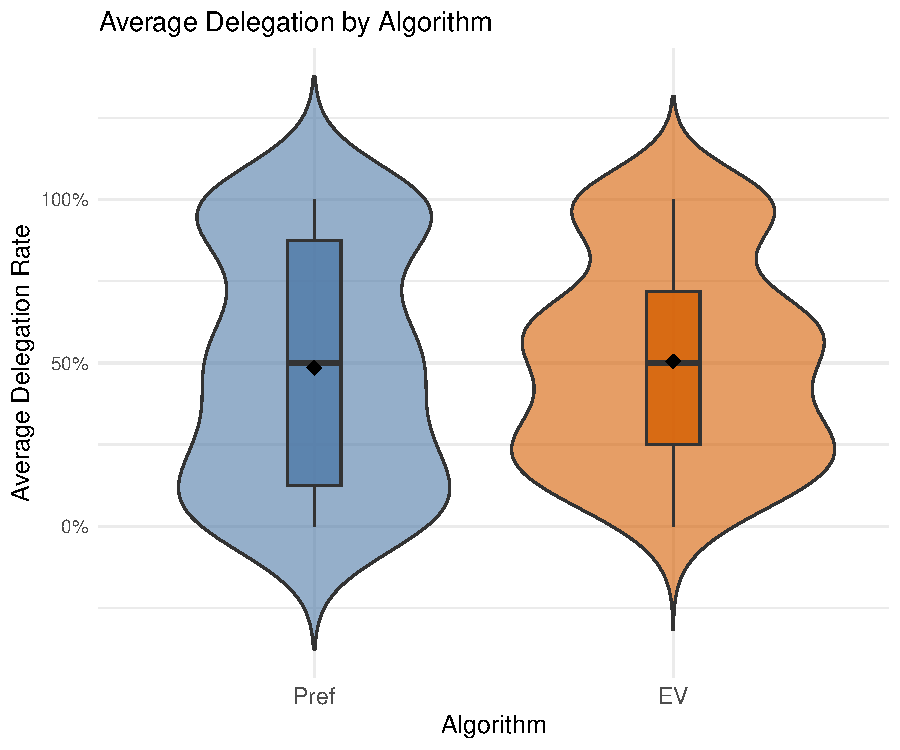
\includegraphics[width=0.78\textwidth]{Figure2_DistributionDelegation.pdf}
\caption{Distribution of delegation propensities across participants.}
\label{fig:delegation_distribution}
\end{figure}

\begin{figure}[htbp]
\centering
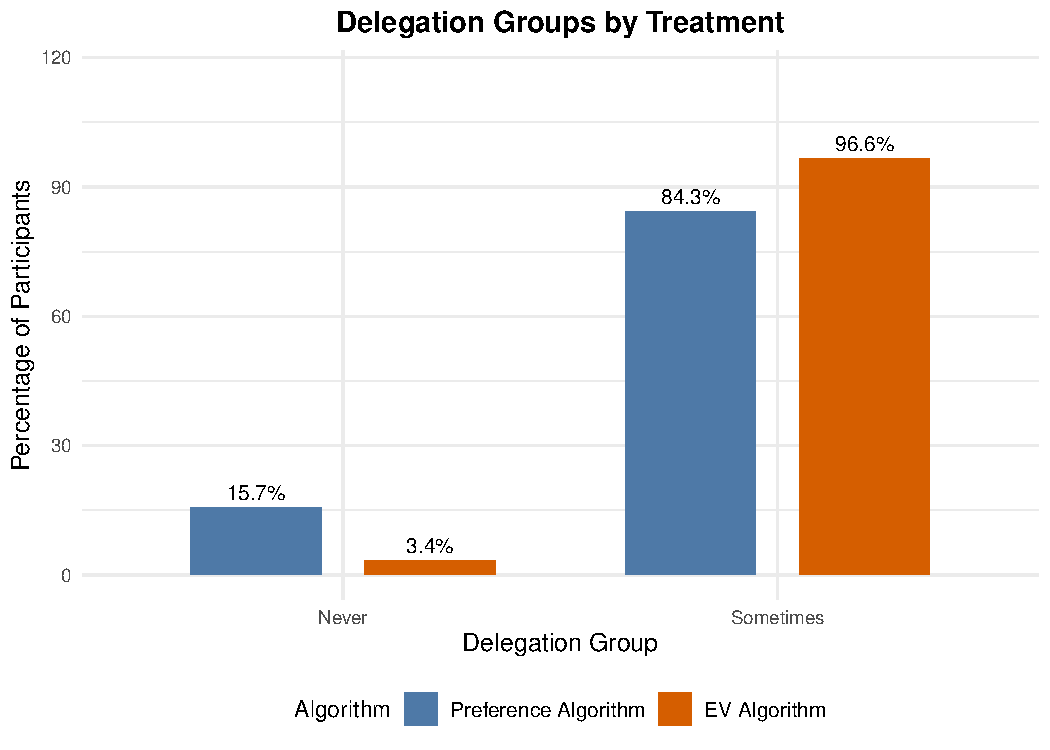
\includegraphics[width=0.78\textwidth]{Figure4_DelegationGroups.pdf}
\caption{Delegation group profiles (never delegators vs. delegators).}
\label{fig:delegation_groups}
\end{figure}

\section{Discussion}
\label{sec:discussion}

\subsection{Main takeaway}
This preregistered study shows that preference-based personalization can deter delegation rather than increase it. The deterrence appears in two forms: lower delegation at first contact and a larger subgroup of participants who never delegate under personalization.

The first-contact finding is theoretically important because it captures behavior before participants can learn from repeated outcome feedback. At that stage, delegation is driven primarily by how participants interpret the algorithmic rule itself. Our evidence is consistent with the interpretation that an impersonal EV rule is initially easier to accept as a legitimate external computation than a profile-based personalized rule that is more self-referential.

\subsection{Interpretation in relation to prior work}
The results refine the algorithm aversion/appreciation literature by moving beyond the human-versus-algorithm comparison and focusing on differences between algorithmic decision rules. Our design isolates a contrast in perceived objectivity and self-relevance, which helps explain why personalization can be normatively appealing yet behaviorally resisted.

The non-delegator pattern is especially informative because aggregate means alone would understate it. A sizable share of the treatment contrast is carried by participants who opt out of delegation entirely when personalization is preference-based, consistent with recent work emphasizing autonomy, responsibility, and control as key moderators of algorithm acceptance. At the same time, the mechanism remains inferential in the present design, because these constructs were not directly manipulated.
This interpretation is consistent with the post-task reason patterns reported in Section~\ref{sec:exploratory_mechanisms}, but those reason measures remain ex-post and hypothetical and should therefore be treated as suggestive rather than causal mechanism evidence.

\subsection{Limitations}
Several limitations should be noted. First, the study is an online experiment with stylized financial lotteries, so external validity to field settings should be interpreted cautiously. Second, although behavioral outcomes are well suited for studying reliance, the design does not directly identify the full psychological mechanism behind first-contact hesitation (e.g., perceived objectivity, profiling concerns, or accountability salience). Third, the present analyses focus on short-run repeated interaction; longer-run adaptation to personalized systems remains an open question.

\subsection{Implications and future research}
For design, the results imply that personalization should not be treated as a uniformly beneficial acceptance lever. In settings where objective criteria are salient and normatively legitimate, objective optimization may face lower initial resistance than preference-based personalization. This has direct implications for the design and communication of decision aids in finance and other high-stakes domains.

Future research should test mechanism-targeted interventions at first contact, including reframing of personalization logic, responsibility framing, and alternative explanation formats. It should also examine whether the non-delegator subgroup is stable across domains, stakes, and cultural contexts.

\subsection{Contributions}
This paper contributes in three ways. First, it provides preregistered evidence that personalization can reduce, rather than increase, delegation at first contact. Second, it shows that resistance is not only transient: personalization is associated with substantially more categorical non-delegation. Third, by comparing two algorithmic decision rules within the same task, it clarifies that behavioral uptake depends on perceived rule characteristics, not only on whether advice is algorithmic.

\subsection{Data and code availability}
Data, analysis code, and study materials will be deposited in a public repository upon acceptance/publication of this manuscript. During peer review, the replication package is maintained in a private repository and will be unblinded and made publicly accessible after acceptance.


\newpage
\thispagestyle{plain}
\addtolength{\topmargin}{-.5cm}
\addtolength{\textheight}{.8cm}

%% \begin{appendices}
% % {\startsupplement
% \renewcommand{\thesection}{Appendix \Alph{section}}
%\renewcommand{\thesubsection}{%\Alph{section}.
%\Roman{subsection}}
%\renewcommand{\thefigure}{}%\Alph{section}.\arabic{figure}}% \Alph{section}}
%\renewcommand{\thetable}{\Alph{section}.\arabic{table}}
%\setcounter{section}{1}
%\setcounter{figure}{0}
%\thispagestyle{plain}

\bibliographystyle{apalike}
\bibliography{library}
 \end{document}
